\chapter{Analýza požiadaviek systému}

Hlavnou úlohou navrhovaného systému je umožniť užívateľovi pohodlne pracovať na odhaľovaní parsovacích vzorov použitím Recursive User-Reviewed Clustering cyklu a algoritmu Extended Nagappan-Vouk. Užívateľské rozhranie musí byť prívetivé a informovať používateľa o~prípadných chybách počas analýzy logovacích správ.

\section{Užívateľské akcie - prípady užitia}

Systém automaticky predpokladá, že užívateľ pri prístupe má v~pláne začat analyzovať logovacie správy. Užívateľ je preto presmerovaný na záložku Miner do stavu začatia novej analýzy. V~tomto stave môže užívateľ zadať zdroj dát, z~ktorého budú pochádzať data analyzované v~ďalšom kroku, alebo tento krok preskočí. Následne môže ako zdroj vstupných dát vybrať logovací súbor alebo použiť nespracované logovacie správy, ktoré sú v~systéme uložené. Dostupné sú aj nastavenia algoritmu, ktoré sú špecifické pre nasledovný beh analýzy. Užívateľovi sú potom prezentované nájdené parsovacie vzory, ktoré sa buď môže rozhodnúť potvrdiť alebo s~nimi ďalej pracovať. Uživateľ si ďalej môže nájdené vzory prehliadnuť, zobraziť správy, ktoré k~nemu patria, poprípade daný vzor odstrániť. Nájdené vzory sa dajú filtrovať podľa zdroja správ a vyexportovať. Dané prípady užitia sú prezentované na obr. \ref{fig:use-cases}, ktorý je nasledovaný detailnejším popisom.

\clearpage

\begin{figure}[htbp]
 \centering 
 \begin{minipage}{0.9\linewidth}
 	\centering
 	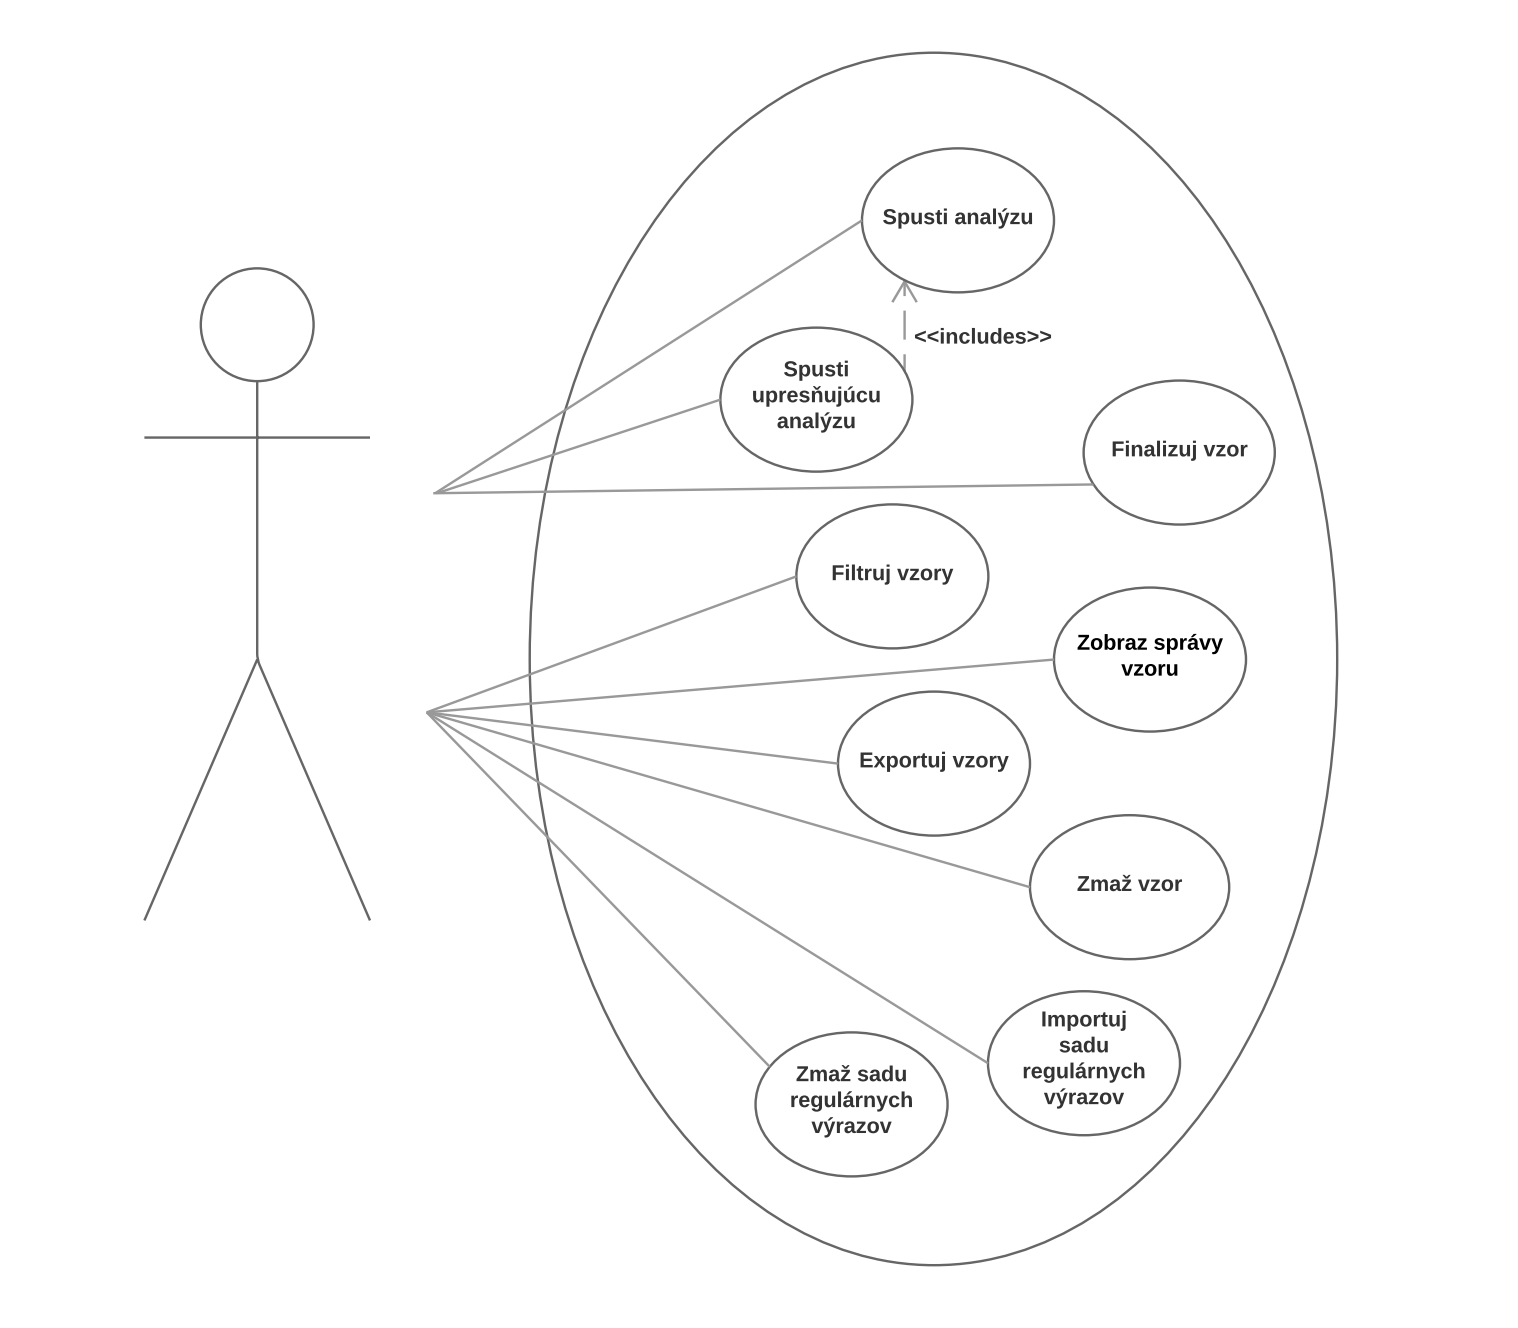
\includegraphics[width=\textwidth]{images/thesis-use-cases.png}	
 \end{minipage}
  \caption{Prípady užitia}
  \label{fig:use-cases}
\end{figure}

\begin{enumerate}
  \item Ako užívateľ zadám vstupný súbor a spustím analýzu.
  \begin{enumerate}
  	\item Po zobrazení užívateľského rozhrania môžem zadať zdroj dát pre nasledujúcu analýzu, alebo môžem tento krok preskočiť.
  	\item Pred spustením môžem meniť hodnotu percentilu a oddeľovačov slov.
  	\item V každom momente môžem začať novú analýzu.
  \end{enumerate}
  \item Ako užívateľ, ktorý už spustil prvotnú analýzu, viem označiť podmnožinu nájdených vzorov a pustiť nad nimi spredňujúcu analýzu
  \item Ako užívateľ, ktorý už spustil prvotnú analýzu, vyberiem nájdený vzor a finalizujem ho.
  \item Ako užívateľ viem filtrovať medzi nájdenými vzormi podľa zdroja dát.
  \item Ako užívateľ viem zobraziť správy, ktoré prislúchajú k danému vzoru.
  \item Ako užívateľ viem zmazať nájdený vzor.
  \item Ako užívateľ viem exportovať nájdené vzory.
  \begin{enumerate}
  	\item Pred exportom si vyberiem sadu regulárnych výrazov, pomocou ktorých sa nájdený vzor prevedie do formátu REtrie.
  \end{enumerate}
  \item Ako užívateľ viem importovať sadu regulárnych výrazov pre export.
  \item Ako užívateľ viem zmazať sadu regulárnych výrazov pre export.
  \begin{enumerate}
  	\item Defaultná sada nejde zmazať zo systému.
  \end{enumerate}
\end{enumerate}

\section{Komponenty systému}
Po preskúmaní požiadaviek sme dospeli k~záveru, že systém vieme ďalej rozdeliť do týchto kategógií:

\begin{enumerate}
  \item Task queue
  \item Webový backend
  \item Úložisko dát
  \item Užívateľské rozhranie
\end{enumerate}

\subsection{Užívateľské rozhranie}
Užívateľské rozhranie musí byť intuitívne a poskytovať dobrú podporu pre asynchrónne operácie, ktoré bude spúšťať. RURC proces definovaný v~\ref{sec:rurc} môže byť v~budúcnosti ešte rozšíreny, preto je zároveň dôležité, aby sa užívateľské rozhranie dalo jednoducho rozšíriť a zdrojový kód udržovať.

\subsection{Webové api}
Backend bude prijímať a spracovávať požiadavky od klienta. Musí vedieť persistovať data, spúštať dlhotrvajúce úlohy na task queue a poskytovať klientovi možnosť zistiť status bežiacej úlohy. Mala by byť použitá dobre známa technológia, ktorá sa dobre integruje a umožnuje rýchly vývoj.

\subsection{Task queue}
Je zodpovedná za beh dlhotrvajúcich operácií. Dôležitá podmienka je stabilita, výkonnosť a schopnosť zotaviť sa z~chyby. Je podstatné, aby po výskyte chyby v~jednom behu úlohy, nebola ovplyvnená schopnosť prijímať ďalšie. Je tu zároveň požiadavka na možnosť dotazovať sa na stav bežiacej úlohy.

\subsection{Úložisko dát}
Dáta s~ktorými sa v~aplikácii pracuje, sú jednoducho štrukturované z~relačného pohľadu. Naviac veľkú časť dát tvoria medzivýsledky, ktoré potrebujeme vedieť rýchlo spracovať a uložiť, ale po krátkom čase už nebudú a zo systému budú zmazané. Preto sa naskytá otázka, či sa má použiť tradičná relačná databáza alebo niektorá z~NoSQL databázi. 

\section{Technologické riešenie}

Extended Nagappan-Vouk algoritmus aj RURC cyklus sú dostupné pod slobodnou softvérovou licenciou. Preto aby výsledný systém bol ľahko nasaditeľný a dostupný, všetky technológie a nástroje použité na implementáciu a beh systému by mali byť pod slobodnou licenciou.

\subsection{Programovací jazyk}
Ako programovací jazyk systému sme po úvahe zvolili Python. Python bol vybraný, pretože už je používany v~existujúcich systémoch ÚVT, bol použitý pri referenčnej implementácii spomínaných algoritmov a dobre sa hodí pre použitie v~našom systéme. Python je rozširený a populárny dynamický typovany jazyk, ktorý patrí medzi základnú sadu programov nainštalovaných na väčšine Linuxových distribúcií. Medzi jeho prednosti patria široká škála voľne dostupných knižníc a jednoduchá správa závislostí, napr. použitím balíčkovacieho správcu pip. 

\subsection{Task queue}
Užívateľ si v~klientskej časti navolí parametre a klient pomocou http volania API spustí algoritmus hľadania parsovacích vzorov.
Dĺžka behu spustenej analýzy je silne závislá od počtu vstupných logovacích správ, ale skoro vždy je to časovo náročná operácia a klientská aplikácia by nemala čakať na response až na jej koniec. Preto je potrebné zvoliť riešenie, ktoré túto analýzu spustí na pozadí a ponúka nám možnosť získať výsledky neskôr. Task queue je systém pre paralelné vykonávanie úloh neblokujúcim spôsobom. Task queue pre svoje fungovanie využíva tieto komponenty :

\begin{enumerate}
  \item Broker, prostredník ktorý drží zadané úlohy.
  \item Producent, funkcia ktorá vytvára úlohy a posiela ich na brokera na neskoršie spracovanie.
  \item Konzument, vezme úlohy z~brokera a vykoná ich. Neformálne si konzumenta môžeme predstaviť ako jedno vlákno, ktoré čaka na spustenie úlohy.
\end{enumerate}

Ako implementáciu task queue sme vybrali celery, v~súčasnej dobe asi najpoužívanejšie riešenie. Celery je dobre zdokumentované riešenie, ktoré je oproti ostatným variantom komplikovanejšie, ale vyniká vo výkone a stabilite. Ako broker sa odporúča využiť RabbitMQ alebo Redis. Vybrali sme Redis, pre jeho možné využitie ako úložisko dát, ako je spomenuté v~\ref{sec:store}.

\subsection{Webový backend}
Pri výbere technológie pre webový backend sme brali do úvahy podporu technológie pre prácu s~celery a následne aj formu, akou bude vytvorené užívateľské rozhranie. Rozhodovali sme sa medzi dvoma najzámejšími frameworkami pre python, konk. medzi frameworkami Django a Flask. Django je viac robustné, poskytuje programátorovi väčšiu podporu, ale aj väčšie obmedzenia. Flask je na druhej strane jednoduchý framework, ktorý necháva programátorovi väčšiu voľnosť. Oba frameworky podporujú pohodlnú prácu s~celery. Nakoniec sme vybrali Django kvôli dobrej osobnej skúsenosti.

\subsection{Úložisko dát}
\label{sec:store}
Pre ukladanie dát sme sa rozhodli použiť kombináciu relačnej databázy PostgreSQL a in-memory databázy Redis. PostgreSQL je open source databáza, ktorá plne implementuje štandard ANSI SQL a spĺňa vysoké nároky na konzistenciu dát a výkon súčasne. Hoci je PostreSQL  rozsiahly systém s~množstvom nastavení pre ladenie výkonu, je veľmi ľahko nainštalovateľná a už v~základnom nastavení poskytuje dobrú výkonnosť. Navyše framework Django odporúča pri výbere databázy použiť práve PostgreSQL, čo považujeme za výhodu. Redis už v~infraštuktúre máme použitý ako broker pre celery. Mimo to je Redis super rýchle in-memory úložisko typu kľúč-hodnota. Poskytuje sadu datových typov, ktorá je postačujúca na uloženie medzivýsledkov a asynchrónne ukladanie dát na disk.
Vo výsledku teda použijeme Redis pre uloženie všetkých neštrukturovaných dát a medzivýsledkov a PostgreSQL prácu so štukturovanými datami. To nám umožnuje dosiahnuť vysoký výkon v~prípade potreby.

\subsection{Užívateľské rozhranie}
Pretože Django poskytuje pomerne dobré templatovacie možnosti, rozhodli sme sa túto možnosť využiť ako základ rozhrania. Ale na dosiahnutie interaktivity a asynchrónnosti je nutné použiť javascript. Vybrali sme preto knižnicu jQuery, ktorá sa ľahko integruje a pracuje dobre v~kombinácií s~Djangom. Týmito technológiami bol vytvorený funkčný prototyp, ktorý odhalil určité nedostatky. Pre naimplementovanie zobrazovania výsledných parsovacích vzorov bolo nutné použiť stromovú štruktúru, v~ktorej sme potrebovali pridávať a odoberať uzly na užívateľom zvolenenom mieste v~strome. Práca s~týmto stromom bola s~knižnicou jQuery síce možná, ale obslužný kód bol zbytočne komplikovaný a zle udržovateľný. Preto sme sa rozhodli túto kombináciu nahradiť čisto javascriptovým riešením. Bola zvolená knižnica Angular 2, ktorá je zameraná na vývoj interaktívnych aplikácií, umožňuje krátky vývojový proces a má veľkú sadu vývojárskych nástrojov.
Na štýlovanie užívateľského rozhrania sme použili Bootstrap. Jedná sa o~momentálne najpoužívanejšie riešenie pre tvorbu moderných a responzívnych webov. To umožnilo, že výsledné rozhranie je z~veľkej miery responzívne, aj keď nepredpokladáme jeho časté využitie na mobilných zariadeniach.

\begin{figure}[htbp]
 \centering 
 \begin{minipage}{0.95\linewidth}
 	\centering
 	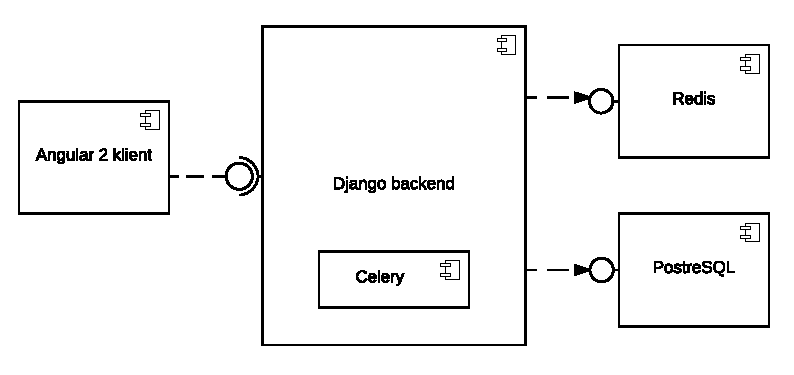
\includegraphics[width=\textwidth]{Images/thesis-component-diagram.pdf}	
 \end{minipage}
  \caption{Komponenty aplikácie }
  \label{fig:components}
\end{figure}

\section{Implementácia systému}
Štruktúru zdrojových kódov sme rozhodli rozdeliť na 3 časti. Serverová časť obsahuje zdrojové kódy v~pythone pre backend a producentov úloh pre celery. Klientska časť zapuzdruje užívateľské rozhranie v~Angular 2 a nástroje potrebné na vývoj a preklad zdrojových kódov. V~inštalačnej časti sú skripty, ktoré plne automatizujú nasadenie aplikácie na linuxový server.